\documentclass{article}
\usepackage{pdfpages}
\usepackage[utf8]{inputenc}
\usepackage[english]{babel}
\usepackage{hyperref}
\usepackage{apacite}
\usepackage{mathptmx}
\usepackage[font = {small, it}]{caption}
\DeclareCaptionLabelFormat{cont}{#1~#2\alph{ContinuedFloat}}
\captionsetup[ContinuedFloat]{labelformat=cont}
\usepackage{subcaption}
\usepackage{float}
\usepackage{fancyhdr}
\usepackage{graphicx}
\usepackage{amsmath}
\setlength{\parindent}{2em}
\setlength{\parskip}{1em}
\renewcommand{\baselinestretch}{1.5}


\fancypagestyle{plain}{
\fancyhf{}
\rhead{Mikkel Werling (201706722) \\ Sebastian Scott Engen (201708490)}
\lhead{The Prospects of Emotion}
\cfoot{\thepage}
}
\pagestyle{plain}

\title{The Prospects of Emotion \\
\large Investigating the modulating effects of emotions on the parameters of Cumulative Prospect Theory
}
\author{Mikkel Werling (201706722) \\ Sebastian Scott Engen (201708490)}
\date{January 2021}

\begin{document}
    \maketitle
    \tableofcontents
    \section{Introduction}
    Prospect Theory stands as a leading model for risky decision making, and has been widely adopted \cite{barberis2013jep} and implemented, with over 60 thousand citations \cite{kahneman1979e}. Whilst the theory is more than 40 years old, a recent large-scale replication \cite{kim2020sr} has shown that the empirical foundations for Prospect Theory replicate exceptionally well.

But whilst the replication proved that the behavioral model had substance and stood the test of time, both the new and the old study left a lot to be considered. Several recent studies \cite{cahlikova2017ee,campos2014role} have now shown that the shape of the Prospect Theory function varies greatly under different affective states. Risk preferences, loss aversion and value estimations all seem affected by emotional context, as all the models parameters have been shown time and time again to vary depending on induced affective state.

As Nobel laureate Herbert Simon introduced with his concept of  bounded rationality, “[...] in order to have anything like a complete theory of human rationality, we have to understand what role emotion plays in it.” \cite{simon1967pr}.

But the current state of research on the effects of emotion on Prospect Theory can be described as limited at best. As the research is still at its early stages, most studies are often narrow in their scope (e.g. only investigating one type of emotion, such as fear) and often not cumulative in nature, as most of the studies published today don’t build on each other's findings. 
In general, positive emotions are understudied and there is yet to be established a shared framework for studying the influences of emotions. 

Following a recent literature review \cite{prietzel2020mrq}, our study sets out to unite previous findings, under a more inclusive and abstracted model of emotion, namely the circumplex model of emotion. Moreover, we set out to run a more comprehensive study that does not neglect parts of the dimensional emotion space, like only studying losses under the influence of negative emotions, hereby serving as the first stepping stone towards building a theoretical model, unifying the Circumplex Model of Affect and Prospect Theory.

For the analysis, we unify the two theories using hierarchical bayesian parameter estimation, as it has been shown to be more precise in its estimates than the frequently used maximum likelihood estimates \cite{nilsson2011jomp}.

    \subsection{Prospect Theory}
    \subsubsection{Prospect Theory and Expected Utility}
    Should I invest in windmills or solar energy? Should I buy this t-shirt or these pants? Should I cross the road or should I stay? 
Decisions are one of the most integral parts of any human life. But decisions are also notoriously hard to predict. The study of human decision making has been a defining topic in psychology as well as economics for decades \cite{nilsson2011jomp}. 

One way of simplifying the complexity of decisions is to make participants choose between simple gambles. Each gamble is described by a monetary outcome ($x_i$) and a probability for that outcome ($p_i$) \cite{nilsson2011jomp}. These gambles could for instance be the choice between Gamble A [\$50, .6; \$-50, .4] or Gamble B [-\$10, .5; \$0, .5]. Gamble A is thus a gamble where you have a 60\% chance of winning \$50 and 40\% chance of losing \$50. In the same fashion, Gamble B is a gamble with 50\% chance of losing \$10 and 50\% of nothing happening. 

Previous economic theories have relied heavily on the assumption that humans choose between these gambles by maximizing expected utility (EU) (e.g., \citeA{savage1972foundations,von2007theory}). This is what also has been dubbed \textit{Homo Economicus}. In the example from above, this would mean that the rational human would choose Gamble A over Gamble B, given that Gamble A has an expected utility of \$10, while Gamble B has an expected utility of \$-5. 
In economics, expected utility has been used as a descriptive theory and not a normative theory (Savage, 1954). That is to say, that the model is taken as an accurate account of how humans make decisions. This has been called into question by numerous theories from psychology. These include decision affect theory \cite{mellers2000choice}, the priority heuristic \cite{brandstatter2006priority} and the dual system model of preference under risk \cite{mukherjee2010dual}. 

The most influential alternative to expected utility, namely Prospect Theory, was published in 1979 by Daniel Kahnemann and Amos Tversky \cite{kahneman1979e}. Instead of assuming that humans are calculating which option is best given objective values and probabilities, Prospect Theory states humans are basing their decisions on subjective values and probabilities instead \cite{kahneman1979e}. This is done by having subjective weights on both values and probabilities. Moreover, Prospect Theory allows for the decision maker to have different subjective weights for positive and negative values \cite{nilsson2011jomp}.
This flexibility in the model has been the major selling point for Prospect Theory, because it enables Prospect Theory to explain systematic deviations from the predicted behavior of individuals under expected utility \cite{nilsson2011jomp}. Most notably, Prospect Theory can accommodate the finding of risk-aversion for gains in high probability and risk-seeking for gains of low probability, as well as risk-seeking for losses of high probability and risk-aversion for losses of low probability \cite{nilsson2011jomp}. In turn, Prospect Theory can explain deviations from expected utility such as the Allais Paradox and framing effects \cite{fennema1997original}.

    \subsubsection{Cumulative Prospect Theory (CPT)}
    Although Prospect Theory can explain previously unexplainable findings from experimental data, the theory in its original form received criticism on its specific mathematical formulation \cite{nilsson2011jomp}. More specifically, the original conception of Prospect Theory was only well-suited for explaining binary outcomes \cite{fennema1997original}. This relates specifically to the problem of stochastic dominance. As probabilities are distorted by the probability weight function $(\pi)$, probability masses are skewed \cite{fennema1997original}. When considering multiple different outcomes in non-binary gambles, too much of the probability mass can sometimes be placed on many different outcomes. It is this overweighting of all outcomes in specific gambles that violates what is called stochastic dominance \cite{fennema1997original}. 
Due to these criticisms, Kahnemann and Tversky proposed a revision of Prospect Theory called Cumulative Prospect Theory (CPT) \cite{tversky1992advances}. CPT solves the issue of stochastic dominance by only overweighting extreme values of gambles, while underweighting intermediate values between these extremes \cite{fennema1997original}. CPT  uses a value function that has the same characteristics as the original value function of Prospect Theory. However, CPT applies a “rank dependent functional” \cite{fennema1997original} for gains and losses separately and sums the two resulting evaluations. This allows the modelling of different weights and functions for losses and gains, reflecting different attitudes for loss and gains in decision makers. 
For our study of decisions, we use cumulative prospect theory instead of prospect theory. This is done to more neatly model functions associated with losses and gains separately. This will be explained in detail in its own section.

    \subsubsection{Replication}
    Tversky and Kahneman’s revised cumulative Prospect Theory model was published back in 1992, and since then several critiques have emerged. An important subset of these are the following: The original experiment did not account for the effects of order in the presentation of lotteries \cite{nwogugu2006amac}, the model is not extendable to real-world decision making and lack areas of applications \cite{rossiter2019jcb}, that Prospect Theory’s experimental setup have prospects confined to either the negative or positive domain, but not mixed prospects that characterize most actual investments \cite{levy2012hotfofdm}, and that Prospect Theory holds a poor replication rate \cite{millroth2019jdm}.

The last critique is especially impactful as it was put forward by a recent large-scale study \cite{millroth2019jdm}. The study found that numeracy could possibly be driving the effects of Prospect Theory. Here participants low in numeracy were making decisions incompatible with the predictions of Prospect Theory, whilst the Prospect Theory function was positively related to the participants' numeracy.

But importantly, a more recent large scale multinational pre-registered study published in Nature 2020 confronted many of these critiques \cite{ruggeri2020nhba}). After having calculated sufficiently powered sample sizes for each country the study set out to evaluate the reproducibility of Prospect Theory in samples with multiple settings and languages. The study had a sample size more than double that of the previous large-scale study and included participants from more than 15 countries. 

First and foremost, the study responded to the criticisms of not having mixed the order of lotteries by including randomization. The study then later concluded that it rendered no effect on the reproducibility of Prospect Theory.

Secondly, the study found an overall replication rate of 94.1\% with all significant effects being in the same direction as the original study from 1979. Whilst this larger study did not measure numeracy directly, it used education as a proxy variable and did not find that low numeracy should code for or drive the effects of Prospect Theory. Moreover, the study found no pattern in terms of higher or lower replication rates based on higher and lower incomes, and neither that any of the demographic variables could consistently predict the choices of participants. 

In response to the critique that Prospect Theory had little replication in the real world, a highly influential literature review from 2010 showed how Prospect Theory has seen a huge effort to be integrated into both finance and insurance where attitudes to risk play a key part in calculations (e.g. calculating the return on stocks and home insurances).
These efforts showcase a different narrative than the critique gave; that Prospect Theory is attractive and is starting to get well integrated into other and more traditional models of economic behavior and real world applications \cite{barberis2013jep}. 

(WHERE ARE THESE REFERENCES?!) Lastly, a well cited study set out to fill the gap of experimental evidence of mixed gambles. Here loss and gains could be compared directly in the mixed condition (See Fig.1)

\begin{figure}[H]
    \begin{centering}
    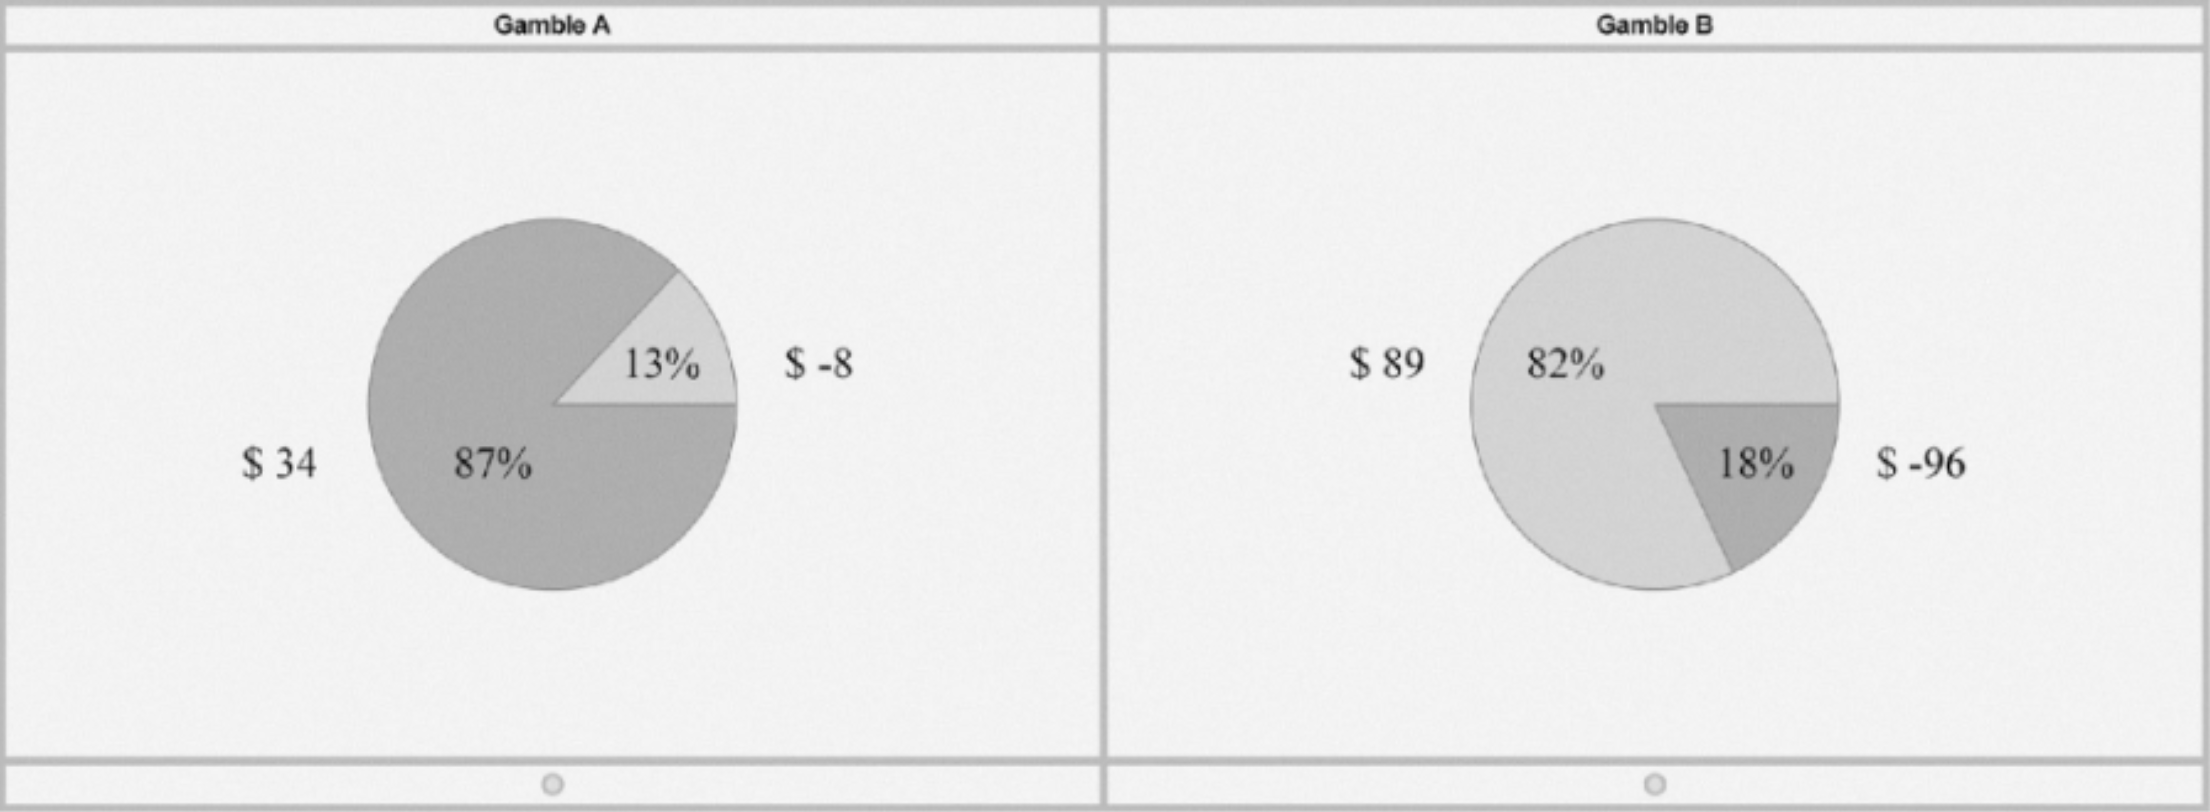
\includegraphics[width = \textwidth]{figures/Billede 1.png}
    \caption{The experimental setup in Nilsson et al., (2011). Adapted from Nilsson et al., (2011)Participants had to choose between the two gambles. This example includes a mixed gamble.}
    \end{centering}
\end{figure}

The study concluded that mixed gamble also followed the predictions made by Prospect Theory. Participants choose the gamble predicted by the model in 98\% of the gamble tasks, including the mixed gambles.

All in all, these findings show the strength and general reproducibility Prospect Theory. 


    \subsubsection{The parameters of Cumulative Prospect Theory}
    Following what we’ve learned concerning the predictive power of Prospect Theory over other models of risky decision making (e.g., EUT), as well as its reproducibility, we’ll now follow the specific coding guidelines for analysis and parameter estimation of Cumulative Prospect Theory, as created and used by \citeA{nilsson2020jomp}, as their Hierarchical Bayesian Parameter Estimation will serve as the basis for this study.

    \begin{figure}[H]
        \begin{centering}
        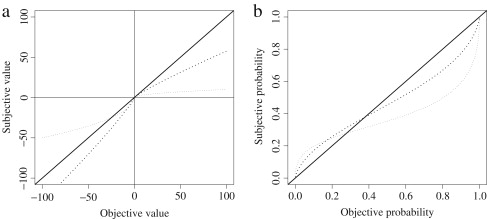
\includegraphics[width = \textwidth]{figures/Billede 2.jpg}
        \caption{Value and probability functions (Adapted from Nilsson et al (2011). a) The plot shows two different value functions as well as the objective value $(x = y)$. The thick dotted line depicts the value function reported in original paper by Kahnemann and Tversky; $\alpha=.88$, $\lambda=.88$, and $\lambda=2.25$. The thin dotted line shows an alternative value function, where all parameters are 0.5; $\alpha=.5$, $\beta=.5$, and $\lambda=5$. b) The plot shows two different probability functions as well as the objective probability function $(x = y)$. The thick dotted line has the parameter $c=.69$ and the thin dotted line has the parameter $c=.5$. Taken together, these functions constitute Cumulative Prospect Theory. }
        \end{centering}
    \end{figure}

    Cumulative Prospect Theory try to present a psychologically plausible explanation for how people estimate the subjective value and probability for prospects with a number of different outcomes, and it is defined by the formula \cite{nilsson2011jomp}:

    $$V(O) = \sum \pi (p_i)v(x_i) $$

    Here the overall $V(\dot)$ describes the perceived prospect of an outcome $(x_i)$ given its probability $(p_i)$, whilst $\pi(\dot)$ and $v(\dot)$ denotes the weighting function for turning objective probabilities and objective values into their subjective counterparts respectively. $i$ denotes the index for each considered value and the probability associated with the value. $\sigma$ describes our sum function. It is the newest addition to the model, the part that was added in 1992, that enables us to have more than 2 gambles presented, and sums these for each trial \cite{tversky1992advances,fennema1997original}.

    The value function $v(\dot)$, which can be defined as:

    $$v(x) = \begin{cases}
        x^\alpha & \text{if } x \geq 0 \\
        -\lambda(-x)^\beta & \text{if } x < 0 
    \end{cases}$$

    First thing we notice is that the model is anchored around a reference point, with v(0)=0, so that the shape of the function for gains and losses will have different shapes. This is captured in the differing functions for $\alpha$ and $\beta$.
Experimental evidence from Prospect Theory has shown that people use a concave function when estimating the value of gains and a convex function when estimating losses. Here the concavity in the gain domain afford risk aversive behavior when dealing with gains, whilst the convex function in the loss domain afford risk seeking behavior for losses (See Fig. 1).
Moreover, we also see the phenomena of loss aversion specified in the negative half of the $\beta$ model, as $\lambda$ codes directly for a drop of the intercept in the loss domain, meaning that small losses are subjectively felt as much larger than the objective value of the loss would indicate.

The probability function $\pi(\dot)$, is defined as:

$$\pi(p_i) = \frac{p_i^c}{(p_i^c-[1-p_i^c])^\frac{1}{c}}$$

Here $\pi(\dot)$ is the subjective weight function, which maps objective probabilities to subjective probabilities. The parameter $c$ codes for an inversely s-shaped transformation of the weighting function (See Fig. 1), and like the value function, it is bound to the specific type of prospect it’s dealing with (Gains or Losses). Each person will transform their probabilities for gains and losses differently, and accordingly the constant $c$ will be substituted for the constant $\gamma$ in the gain domain, and the constant $\delta$ in the loss domain.

Both of these constants are values between 0 and 1, and specify the curvature of the function.
Findings have shown that lower probabilities generally are overweighted, whilst higher probabilities are underweighted, as depicted in the dotted line in Fig. 1.  Importantly, it has been found that $\gamma$ and $\delta$ differ in subjects, suggesting that the subjective weighting varies across the domains of gains and losses.

An important note is that Cumulative Prospect Theory is a deterministic model \cite{nilsson2020jomp}. By this we mean that subjects are expected to choose the option with the largest value. However, this does not account for the probabilistic features of human decision making, where people often deviate from predictions \cite{nilsson2011jomp}. To accommodate this, we add an error theory to our model, specifying the extent to which a participants choice is determined by their value function \cite{nilsson2011jomp}:

$$p(A,B) = \frac{e^{\varphi(V(A))}}{e^{\varphi(V(A))} + e^{\varphi(V(B))}} $$

The $\varphi$-parameter in other words denotes how random the behavior of individuals is. Higher values of $\varphi$ indicate that behavior is more determined by their value function. This ranges from 1 to 0, where 1 is perfectly determined and 0 is perfectly random. 
 
The specific formulation of the Cumulative Prospect Theory model we will use in this paper includes 6 parameters, each of which is directly interpretable from the model outputs of the model by \citeA{nilsson2020jomp}.
They are as follows:
$\alpha$ defines the concave curvature of the subjective value function in the gain domain;
$\beta$ defines the convex curvature of the subjective value function in the loss domain;
$\lambda$ defines loss aversion;
$\gamma$ defines the probability weighting function’s shape in the gain domain;
$\delta$ defines the probability weighting function’s shape in the loss domain
$\varphi$ defines to what degree choice behavior is determined by subjective values.


    \subsection{Emotions}
    \subsubsection{Rationality and Emotions}
    Prospect Theory marked the birth of behavioral economics, as it laid bare how and why classical Rational choice models (e.g. Expected Utility) had low predictive power. The models put forward by Kahnemann and Tversky showed that accounting for subjective value estimations could account for much more variability in people’s decision-making behavior. Today the impact of the transition is clearly outlined in the number of public economics papers \cite{kleven2018} (See Fig: 2).

    \begin{figure}[H]
        \begin{centering}
        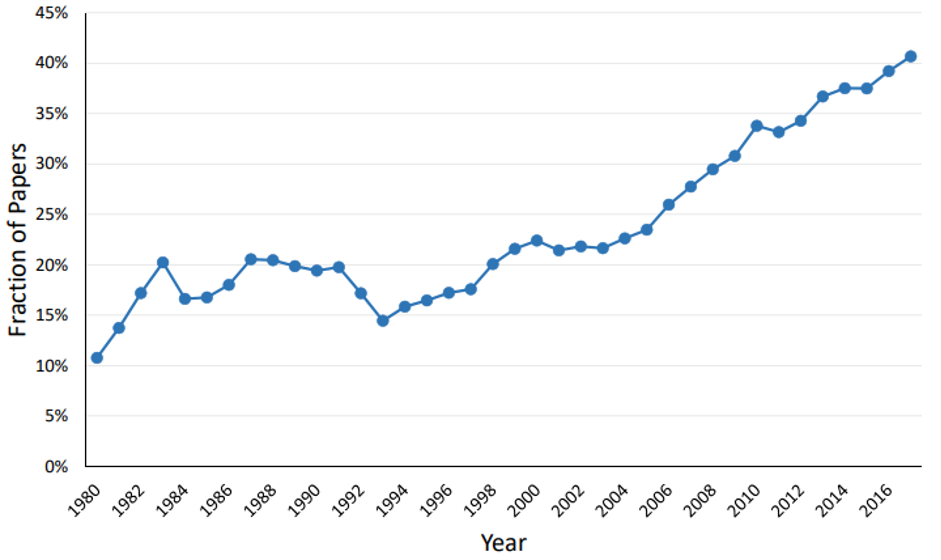
\includegraphics[width = \textwidth]{figures/Billede 3.png}
        \caption{Adapted from Kleven, (2018). The fraction of public economics papers that mention any word unambiguously related to the topic of behavioral economics from 1980 to 2017}
        \end{centering}
    \end{figure}

    But forty years have passed, and more innovations are happening that need to be accounted for. Specifically, the research field of emotion has taken a backseat since the Skinnerian behaviourism retired in 1974, leaving no journal entries on how emotion and decision making relate to each other. As the cognitive revolution rolled out in the following decades, the focus was on rational cognition, and emotion was often deemed irrational and treated more or less as noise in models \cite{barrett2019historical}.
 
But, since the beginning of the 21st century the research landscape has shifted and change is underway in the field of emotion. This is clearly showcased in growth of the proportion of scholarly publications using both the keywords “decision making” and “Affect”/”Mood”/“Emotion” from 1970 to 2013. (See. Fig 2)
    
\begin{figure}[H]
    \begin{centering}
    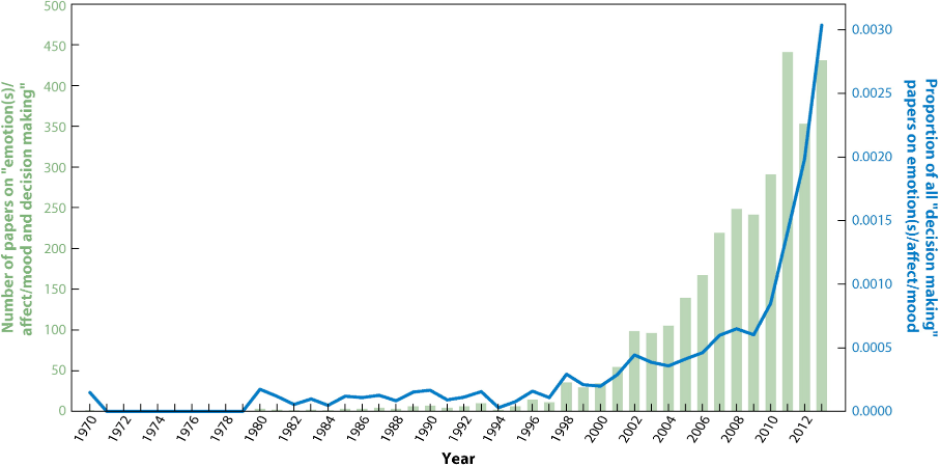
\includegraphics[width = \textwidth]{figures/Billede 4.png}
    \caption{Adapted from Lerner et al., (2015). The fraction of public economics papers use both the keywords “decision making” and “Affect”/”Mood”/“Emotion” from 1970 to 2013.}
    \end{centering}
\end{figure}

As a review from 2010 put it “Decisions can be viewed as a conduit through which emotions guide” \cite{keltner2010emotion}. And whilst decisions often have objective measures of adaptiveness, once decisions are actually made, emotions will follow. Here they serve as at least part of the internal feedback loop that updates and informs a subject about the world.  
 
One example of how emotions can serve as an integral part of decision making comes from a study showing how sadness increases people’s risk aversion in the gain domain of Prospect Theory, whilst also boosting people’s risk seeking behaviour in the loss domain \cite{campos2014role}. This study also shows how another categorical emotion, anger, intensifies the tendency for risk-seeking behaviour in the loss domain, decreasing the parameter for loss aversion by more than 40\% (See Fig. 4).

\begin{figure}[H]
    \begin{centering}
    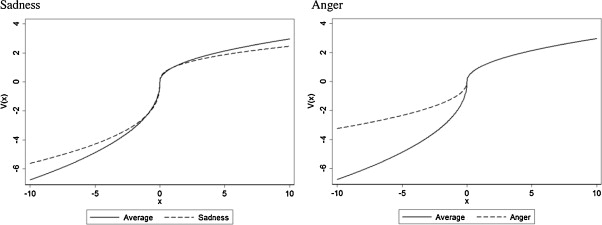
\includegraphics[width = \textwidth]{figures/Billede 5.jpg}
    \caption{Adapted from Campos-Vazquez \& Cuilty, (2014). The graphs show the separate effects of sadness and anger on the Prospect Theory utility function.}
    \end{centering}
\end{figure}

In sum, the science of how emotion and decision making are getting more and more entangled with each other and preliminary evidence indicated just how some aspects of emotion can modulate the utility functions of individuals.
 
Yet, before we can explore the full literature of how emotions shape the Prospect Theory utility function, we will have to get an overview of how the research landscape of emotion looks today.

\subsubsection{Historical shift in understanding emotions}
The field of emotion has a long history with a stable paradigm that we’ll be referring to as The Classical View of emotion (CV).
CV is based in the locationist/modular approach to neuroscience, and has divided emotion up into a distinct set of categories that involve typical physiological expressions as well as specific brain area activations \cite{ekman1976pictures,fodor1983modularity}. These categories of emotions are typically spoken about as the ’Basic Emotions’, and although the exact number of these basic emotions has fluctuated over time \cite{liao20192imimbci}, we will use one definition in this study; namely that of a leading emotion researcher Paul Ekman that has described them as: Anger, disgust, fear, sadness and joy \cite{dalgleish2000handbook}.
 
But modern theories are spearheading critiques against the idea of Basic Emotions and have changed the research paradigm of CV. Since the early 19th century, CV has time and again mapped their a priori defined emotion categories onto both organs and differing brain regions. 
The newer theories, such as the Constructed View of Emotion (CV2), reject this practise of compartmentalizing and concluding on a priori reasoning, to instead restart the theorizing process to include the latest insights about the functional and structural organization of the brain \cite{barrett2019historical}. The new line of research can be seen in several large meta-analytic studies \cite{kober2008functional,lindquist2012brain} as well as studies outlining some of the general advances in neuroscience \cite{smitha2017resting, touroutoglou2015intrinsic}. 
 
To give one concrete example of what tenets of CV are being challenged we have to look no further than to the implicit assumption of modularity \cite{fodor1983modularity}.
Newer network studies, driven by advances in computer processing speed, highlight how most Basic Emotion regions are not unimodal and specific to one emotion, but encode complex combinations of distributed information and serve in processing various tasks and emotions \cite{chang2017code,rigotti2013importance,somerville2006prior,wright2008emotion}.
To give an example of what these studies show, we can zoom in on some of the proposed basic emotion brain regions (e.g. the amygdala and the anterior cingulate cortex) that have been treated as the seat of fear and anger respectively. Here, one study shows that brain areas often work in concert across multiple emotional states, by finding heightened amygdala activity both in emotional instances of fear, anger and more, which is directly  incompatible with the CV’s assumption of specificity \cite{menon2015salience, touroutoglou2015intrinsic}.
 
To give a second example, a recent meta-analysis showed that no instance of induced emotion showed specificity to any of the five basic emotion areas \cite{lindquist2012brain}. Moreover a review of the literature of intracranial electrophysiology concluded the same \cite{guillory2014exploring},  and so did another review of the literature of animal research \cite{barrett2007mice}.
 
All in all, the research landscape seems to be on the brink of monumental change and it is no longer justified to assume one-to-one mappings between specific emotion categories and topographically distinct brain regions \cite{barrett2019historical}.
 
In this study we will therefore move away from the CV’s definitions of emotion, where emotions belonging to a set number of emotion categories. Instead, we will make use of a more abstract model for emotion; the Circumplex model of affect \cite{russell1980circumplex} (See Fig. 5). The Circumplex model of affect accounts for emotion in a more granulated fashion. Here varying emotional experiences are placed inside a dimensional space with the two dimensions: Arousal and Valence. 

\begin{figure}[H]
    \begin{centering}
    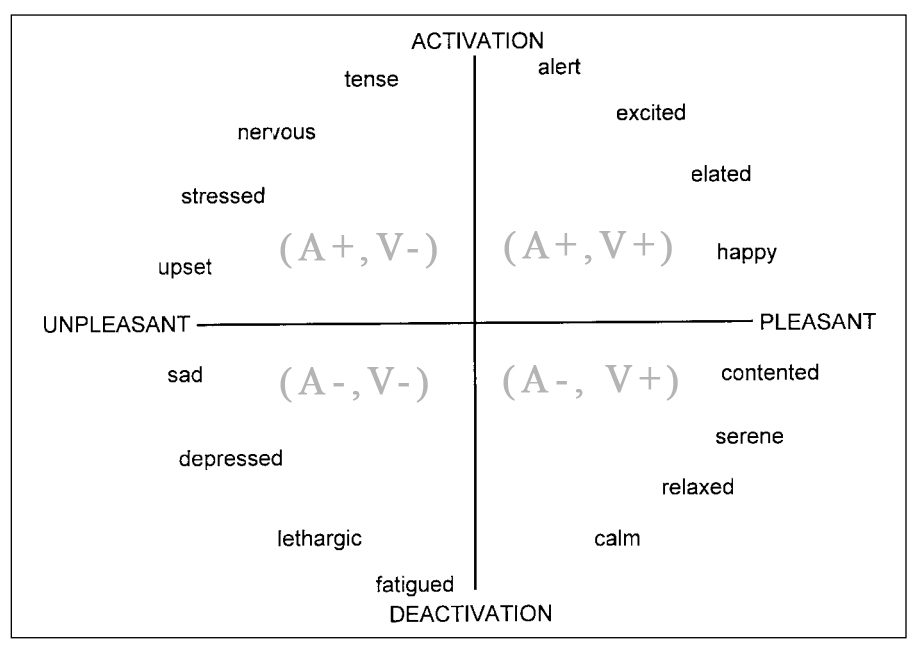
\includegraphics[width = \textwidth]{figures/circumplex.jpg}
    \caption{Adapted from Barrett \& Russell (1999). The plot shows the Circumplex model of affect. The model conceptualizes emotions as being points in two dimensions. The x-axis describes the valence of the emotion, while the y-axis describes the arousal of the emotion. The gray text is the labels for each quadrant of the model. }
    \end{centering}
\end{figure}

Specifically these two dimensions give us four quadrants in the dimensional space and each will serve as one of our four conditions:
\begin{enumerate}
    \item High Valence and High Arousal words (A+V+)
    \item Low Valence and High Arousal words (A+V-)
    \item High Valence and Low Arousal words (A-V+)
    \item Low Valence and Low Arousal words (A-V-)
\end{enumerate}
 
This framework serves as being more robust moving forward, as it can encapsulate older study’s findings inside the dimensional spaces four quadrants (e.g. Anger, that has been shown to modulate loss aversion can be placed within the high arousal/High valence quadrant). It also allows for more diversity in experiences as the model circumvents having to reduce the model space to arbitrary categories. This is important as these categories often vary from study to study.

    \subsubsection{Eliciting Emotions}

    To study how emotions influence behavior, research has primarily been focused on manipulating the emotional state of participants using what is called affect induction procedures (AIP) \cite{joseph2020pbb}. AIP is used as an umbrella term for paradigms, which present participants with stimuli of different types (e.g. text, images, videos), which is thought to influence the affective state of participants systematically. Today it stands as one of the central paradigms used to test theories related to moods and emotions \cite{joseph2020pbb}. It is important to mention that the effect of the affect induction procedure is heavily determined by what stimuli participants are shown. It is therefore tantamount for any experiment using AIP to validate their stimuli. To this end, a recent meta analysis tested the robustness of AIP using 874 samples, covering in total 53.509 participants \cite{joseph2020pbb}. Several of their findings are of interest to this paper. Firstly, they find that overall AIP procedures are on average effective in eliciting an emotional response \cite{joseph2020pbb}. Furthermore, the meta analysis compared the strength of different types of stimuli and found that videos with instructions were the most effective \cite{joseph2020pbb}. For instance, it has been found that explicitly asking participants to watch carefully and feel closely what their affective state is while watching the video is predictive of a stronger emotional response \cite{joseph2020pbb}. This is in line with other research showing that active engagement by participants is vital for a strong emotional response to the stimuli \cite{out2020gradual}. 
What is also of specific interest to this paper is a negativity bias reported in the meta analysis \cite{joseph2020pbb}. In general, negative emotions are more easily elicited in participants than positive emotions. We will explore the effects of this negativity bias in the exploratory section of this study. 

But, concerning the main analysis, we will be using videos with accompanying instructions, asking participants to actively engage with the stimuli, as the emotion elicitation paradigm for this study.

    \subsubsection{Videos}
    As mentioned in the previous section, the most effective AIP material is videos with instructions. But as researchers, we are interested in which videos are most reliably predictive of the induced affective states. In \citeA{gilman2017br}, the researchers sought to find the most effective video material to induce specific emotions. \citeA{gilman2017br} created a database of videos on the basis of a literature review of 24 studies. The resulting videos were sorted in terms of how reliable they elicited emotions in healthy participants. Furthermore, the videos are specifically categorized in terms of arousal and valence, corresponding to the different quadrants of the Circumplex model of affect. 
For our study, we use this database and the videos that were most effective in eliciting emotions in subjects. We include the three most effective videos for each condition, resulting in 15 different videos in total. 

    \subsection{Prospect Theory under the influence of Emotion}
    Alike what was introduced in the section on ‘Rationality and emotion’, several other studies have found effects of the negative emotion Anger on the risk-seeking behaviour in the loss domain \cite{prietzel2020mrq}. This is one amongst many effects that’s been outlined a recent review of the literature on Prospect Theory under emotion. It is important to note that the previous studies have used categorical emotions (e.g. Anger) in their AIPs. To investigate this using the circumplex model, we therefore need to find patterns in the results found from multiple studies. 
One of the studies' several conclusions was that there is yet to be defined an overarching model of how the parameters of Prospect Theory are influenced by emotions. As introduced in the section ‘Emotion’, we propose using the Circumplex model of affect, as it enables us to use and build on the effects found by studies of varying experimental paradigms. For example will we code the direction of effect for studies investigating anger as being Highly arousing and Negatively valenced.
A second conclusion that we intend to build on is that positive emotions are understudied compared to negatively valenced emotion studies. To build on this insight we will have an equal number of participants in each of our four conditions, that accommodate our four quadrants of the Circumplex Model of Affect.

Because of the lack of a systematic approach to investigate emotions and their effect on the parameters of Prospect Theory, there are several unexplored avenues of research \cite{prietzel2020mrq}. As such, previous studies do not enable us to make informed hypotheses on the direction of effect. Specifically, the dimension of arousal has been largely neglected in previous studies \cite{prietzel2020mrq}. When this is said, there are still some general patterns where a reasonable directional hypothesis can be stated. This is the case for emotions of positive valence and their effect on loss aversion. \citeA{prietzel2020mrq} found that across multiple studies considered, emotional states of positive valence resulted in higher degrees of loss aversion. Mathematically, this corresponds to higher values of lambda for both conditions in our experiment associated with positive valence (V+, A+; V+,A-). 
Instead, it is true to conclude that the current picture is murky. This is largely due to binning emotions into categorical labels, as well as previous studies focusing on only one emotion’s effect on the parameters. We therefore think it is reasonable to assume that we will find an effect of an elicited emotion on all parameters, although we do not find indications that we should expect a clear direction of effect given the literature \cite{prietzel2020mrq}. This is especially the case for negatively valenced emotions, where effects differ wildly. We suspect that one reason for the difference in effects is because research has not included the dimension of arousal. By including arousal in our study, we hope that we can find more clear patterns, especially in the negatively valenced domain. 

    \subsection{Models and Procedure}
    \subsubsection{Estimating parameters}
    To model the specific parameters for CPT, previous studies have relied on maximum likelihood estimates of single-participants \cite{nilsson2011jomp}. This approach has been successful in estimating the parameters of CPT specifically when the number of participants is large \cite{harrison2009expected}. However, modelling using single-participant maximum likelihood estimates does have its downsides. The implicit modelling assumption is that all participants are unique, and information about the parameters of other participants are not used to inform the model \cite{nilsson2011jomp}. 

It is often more useful to assume that although participants do differ in the behavior, there will be similarities between them. This can be modelled by letting the parameters for each participant be drawn from a group-level distribution of the parameters \cite{nilsson2011jomp}. Utilizing this approach, the parameters of the individual is informed by the information obtained from the group as a whole \cite{nilsson2011jomp}.

Moreover, the resulting parameter estimation is often given as a point estimate and analyzed further in analysis of variance in order to check for significance between groups. This throws away much of the information regarding the precision with which the parameters have been estimated. This becomes especially critical for the parameter estimation of CPT, which often tends to be relatively uncertain. Throwing this information away allows for unrealistic and extreme values for parameters to be included in the model, which might lead to false conclusions \cite{nilsson2011jomp}. 

Instead of modelling each participant as a unique entity, participants in a hierarchical bayesian framework can be modelled as being samples from the same underlying group-level distribution. This approach offers a compromise between seeing participants as completely unique (single-participant estimates) and completely identical (complete pooling) \cite{nilsson2011jomp}. The problem of point estimates are also circumvented using this approach. In maximum-likelihood approaches, some of the unrealistic and extreme parameter estimates might skew the results \cite{nilsson2011jomp}. Using the hierarchical bayesian framework, all results are partially pooled towards the mean. The more extreme a result is, the more it will be pooled towards the mean. This is especially useful for estimating parameters of high uncertainty, which is the case for CPT \cite{nilsson2011jomp}. 

    \subsubsection{Bayesian Approach and Results}

    Beyond making more reasonable assumptions in our model, adopting a bayesian approach has other advantages. 
Of particular importance for our intents and purposes is that Bayesian statistics has been shown to be more robust to the “family-wise error” associated with multiple tests \cite{sjolander2019frequentist}. This pertains to our study, as we will be testing differences between the baseline and four different conditions. In these tests, we will investigate all the six different parameters, which amounts to 24 different tests. It is therefore vital for our inferences that we consider that differences will be pronounced in our data by sheer chance. 
In sum, we adopt a hierarchical bayesian framework to implement partial pooling of the parameter values of each group (condition) and to circumvent the problem of multiple comparisons.
\\
Along these lines, an advantage of the Bayesian approach is that unlike frequentist inferences, we are not solely concerned with rejecting the null \cite{sjolander2019frequentist}. In a Bayesian framework we use the data to build a case for our alternative hypotheses, compared to the null, whilst if using frequentist inferences, we in principle are only concerned with disproving the null \cite{sjolander2019frequentist}. 

Since we are dealing with many hypotheses, we opt for the bayesian approach, specifically because it allows us to assess if our data favors the null compared to our hypotheses. 

The Bayesian approach does however have some downsides. Specifically, power analyses can be done in many ways with different levels of conservatism. In contrast, a frequentist framework would be able to calculate this formally. We decided to use a threshold which mirrors the intuition from a frequentist perspective. Here, we are specifically referring to the nominal 0.8 statistical power, which describes being able to reject the null-hypothesis 80\% of the time if there is an effect to be found. The specific power analysis performed is described in detail in its own section and all the code is available on \href{https://github.com/sebsebar/Nature-Study/blob/main/PowerAnalysis/BayesianPower.Rmd}{Github}. 

    \subsection{Hypotheses}
    Our hypotheses fall into three distinct parts. These three parts reflect (1) the validity of our manipulation (2) the validity of the results in a novel online domain and (3) how the manipulation specifically interacts with the parameters of cumulative Prospect Theory.
    \subsubsection{Manipulation checks}
    To check for a stimulus-driven effect on overall arousal and valence (e.g., that high vs low arousal video stimuli increase arousal differently), we will have the participants rate arousal (on a scale 1 - calm to 9 -excited) and valence (on a scale 1-unhappy to 9 - happy) of the words using Self-Assessment Manikin (SAM) \cite{bradley1994measuring}. SAM has been used to a large degree in the literature and has been validated as an efficient tool for extracting points on the circumplex model SAM \cite{bradley1994measuring}. Our hypothesis for these results is that the previously validated emotion elicitations will elicit similar evaluations in our participants. We will take similar elicitations to mean that participants fall into the same quadrant of valence and arousal as the videos have previously elicited in other populations. 
    \subsubsection{Cross study check}
    First, we want to investigate whether the previously reported findings using the same paradigm can be validated with new data. We therefore include what we call the baseline condition. The baseline condition follows the exact analysis and stimuli used in Nilsson et al. (2020). This serves as a first robustness measure. This first replicability test will ensure that the paradigm and the analysis shows the same overall patterns which have been found reliably in the literature (e.g. Loss Aversion). 
Second, we will also check the generalizability of the results in a novel domain. Specifically, we will run the same study in an online setting. This will allow us to comment on whether the previously reported parameters of cumulative Prospect Theory are robust to changes in experimental setting. 
The baseline conditions of these two studies will serve as a sanity check for whether our findings are in line with the existing literature. Importantly, they will also allow us to investigate whether the interaction effects between the parameters of cumulative Prospect Theory and emotions are robust across online and offline domains. 

    \subsection{Hypothesis testing}
    Our primary interest is the effects of AIP on the parameters of Cumulative Prospect Theory. We conceptualize emotion elicitation to fall into positive and negative values over the two dimensions of Valence (V) and Arousal (A). This gives us four distinct conditions in addition to the previously mentioned baseline: (V+,A-), (V+,A+), (V-, A+) and (V-, A-). We will test our hypothesis for each parameter as deviations from the baseline condition. This enables us to look at the main effect of valence and arousal, as well as interaction effects of specific combinations of the two dimensions. 
    Our principal tests of interest will be a repeated measures 2x2 factorial design (Arousal by Valence) of the cumulative Prospect Theory function on mixed gambles. First, the parameters of cumulative prospect theory ($\alpha, \beta, \gamma, \delta, \lambda and \varphi$) will be estimated using a Hierarchical Bayesian Parameter Estimation. From this function we’ll be able to find mean parameter estimates as well as the uncertainty of that estimate (standard deviation). 
    Taken together, the mean and the standard deviation constitutes a distribution. We will use Bayesian T-test/ANOVA to check the probability of the alternative hypothesis given the data. This will specifically be calculated using Bayes Factors.
    \subsubsection{Null Hypothesis: No effect of Emotions on Prospect Theory}
    Under the null hypothesis, we expect to observe no effects of stimulus arousal or valence on the parameters of Prospect Theory. This would imply that Risk-Aversion, Risk-Seeking, Loss-Aversion are insensitive to emotional inputs. We take this to be highly implausible, as previous literature has already suggested close ties between emotion and the perception of value and probability (See the section: Prospect Theory under the influence of Emotion).    
    \subsubsection{Alternative Hypothesis 1: Directional Predictions}
    \begin{itemize}
        \item \textbf{Positive Valence gives a higher value of $\lambda$}\\
        Under this hypothesis, we expect to see a main effect of stimulus valence on the directional effects of $\lambda$. This would suggest that valence serves to modulate the loss aversion of the Prospect Theory function. This hypothesis will be supported if there is main effect of valence that renders a Bayes Factor higher than 3 for the positively valenced conditions compared to the neutral baseline. 
    \end{itemize}
    
    \subsubsection{Alternative Hypothesis 2: Non-Directional Predictions}
    Using the parameter estimates from \citeA{nilsson2011jomp}, we are specifically targeting our study to the parameters of Cumulative Prospect Theory associated with the utility function ($\alpha, \beta$, $\lambda$). This was done as the realistic amount of participants (60) is enough to find interesting deviations from the baseline (See the section: Power Analysis). The parameters associated with the probability weighting function ($\delta, \gamma$) were found to have larger uncertainty in their estimates, and therefore require large effects to be found reliably.
Additionally, it is worth stating that our hypotheses for the non-directional effects are categorised into 3 separate hypotheses. We will first investigate the interaction between Arousal and Valence for each parameter. This is referred to as Alternative Hypothesis 2A. If the interaction effect is not pronounced for the particular variable, we will instead investigate Alternative Hypothesis 2B and 2C. 

\begin{itemize}
    \item \textbf{Alternative Hypothesis 2A: An interaction between Valence and Arousal mediates an effect on our parameters}\\
    Under this hypothesis, we expect to see an interaction effect of stimulus arousal and valence on the values of $\alpha, \beta, \lambda, \gamma$ and $\delta$.  To this effect the Prospect Theory parameters for high arousal items will be different for positive-valence items than for the negative-valence items.
    \item \textbf{Alternative Hypothesis 2B: Arousal-Mediated changes in the effects of our parameters are Independent of Valence}\\
    Under this hypothesis, we expect to see a main effect of stimulus arousal on the effects of $\alpha, \beta, \lambda, \gamma$ and $\delta$ with no interaction of stimulus valence. This hypothesis will be supported if there is main effect of valence that renders a Bayes Factor higher than 3 for the positively valenced conditions compared to the neutral baseline.
    \item \textbf{Alternative Hypothesis 2C: Valence-Mediated changes in the effects of our parameters are Independent of Arousal}\\
    Under this hypothesis, we expect to see a main effect of stimulus valence on the effects of $\alpha, \beta, \gamma$ and $\delta$, with no interaction of stimulus arousal. This hypothesis will be supported if there is a main effect of arousal that renders a Bayes Factor higher than 3 for the positively valenced conditions compared to the neutral baseline.

\end{itemize}

    
    \section{Design Plan}
    We will investigate the interaction between elicited emotions and the parameters of cumulative Prospect Theory in two experiments. One experiment will be an online study, conducted on the Qualtrics survey platform, meaning that no researcher will be physically with the participants when they do the experiment. The justification for using Qualtrics as our data gathering website over other similar sites such as MTurk is that the quality of the data is generally considered better on Qualtrics (ref). 
The other study will be an in-lab study in CobeLab in Aarhus, Denmark. These two experiments are identical in all other aspects. 

    \subsection{Blinding}
    As participants are shown videos, and are asked specifically how the videos influence them, it is not possible to effectively blind the participants in terms of which condition they are in. As the participants have no knowledge of other conditions, we do not think this will be a problem for the analysis. To counter any effect of researchers influencing the participants in the in-lab study, the personnel will be blinded to what conditions the participants are in. Furthermore, we follow recent advances in experimental psychology, which also blinds the data analyst. This is done by randomly assigning all conditions with dummy labels, except for the baseline. This will inhibit the data from being tampered with to support the hypotheses, but keeps some flexibility in excluding bad data \cite{dutilh2019flexible}. 
    \subsection{Study Design}
    The experimental design is a within-subject 2 by 2 factorial design. These are the factors: 
\begin{enumerate}
    \item High Valence and High Arousal words (A+V+)
    \item Low Valence and High Arousal words (A+V-)
    \item High Valence and Low Arousal words (A-V+)
    \item Low Valence and Low Arousal words (A-V-)
\end{enumerate}
Each participant will complete 3 blocks of two phases and there will be no breaks in between each block. Phase 1 is the stimulus phase where the participant will watch one of 3 AIP videos for their specific condition (E.g. A+V-). Subsequently, participants will rate their affective state on a 9-point digital Self-Assessment Scale (SAM), to be used as a manipulation check. 
Phase 2 is the task phase, where participants will make 60 two-alternative forced-choice judgment tasks for item pairs, where participants are asked to choose which of two gambles are preferable. 
The entire experiment takes approximately 30 minutes, but there’s no time limit for response time.

The lab-based study will be carried out using PythonScript Editor PsychoPy, whereas the online experiment will be using the online survey platform Qualtrics’s native survey tools.

Both the online and the lab-based study will include a fifth group, exposed to neutral stimuli material. This will serve as a baseline to all the modulatory effects of the four conditions. Moreover, it will serve as a validation test case for the Prospect Theory computed in the paper by \citeA{nilsson2020jomp}.

For the In-lab study, participants will be tested over two consecutive weeks (14 days) in April, 2021. The online study will also start up in April, but run until the target of 175 participants have successfully performed the experiment (See the section: Stopping Rule)

    \subsection{Randomization}
    In this study we will use several layers of randomization.
We will use block randomization, where each participant will be randomly assigned to one of the four equally sized conditions (A+V+,A+V-,A-V+,A-V-).

Within each condition we will adapt the experimental setup so that both stimuli and task phases alternate randomly across blocks. That means that the order of the stimuli phases (Phase 1) within a condition varies across the 3 blocks. The same goes for the 3 groups of gambles (Loss, Gain or Mixed domain) that will also be randomly distributed across the 3 blocks. 

Moreover, each gamble pair position will be randomized across the 60 trials within each block. Each participant will encounter all gamble pairs.
We will use the same gambles as \cite{nilsson2011jomp}. All lottery probabilities was simulated randomly within a spectrum from 0 to a 100. All gamble values will also be simulated randomly. Here values range from 1 to a 100 in the gain domain, -1 to -100 in the loss domain, -100 to 100 in the mixed domain.
    \section{Sampling Plan}
    As of the date of submission, the data has not yet been collected. Keeping this in mind we have access to the prior work of \citeA{nilsson2020jomp}. This becomes relevant for our study as we compare our results from the baseline conditions with the results reported in \citeA{nilsson2020jomp}. 
We rely on this as a sanity check for our results and as to validate our hierarchical bayesian baseline model. 

    \subsection{Data Collection Procedures}

    For the online study, participants (n=69) will be recruited and managed through Qualtrics; a web-based tool to conduct survey research. Here participants must also be at least 18 years old, give written consent, and fluent in English. The participants will be paid by the standard of 50 DKK per hour and the estimated total duration of the test session is 0,5 hour (25 DKK). 

For the in-lab study, participants (n=69) will be recruited through advertisements via Sona system (CFIN) from Aarhus University as well as via social media (Facebook and Twitter). The study will be run in Cognition and Behavior Lab (COBE-Lab) at Aarhus University, and being university based, we expect the majority of our participants to be students. In any case, participants must be at least 18 years old, give written consent, and be fluent in English. 
Per standard, participants will receive 100 DKK per hour for the total estimated duration of 0.5 hours (50 DKK).

The procedures will be conducted following the Declaration of Helsinki and the in-lab study will not be carried out before having received approval from the Danish Neuroscience Centre’s (DNC) Institutional Review Board.

    \subsection{Sample Size}

    \begin{figure}[H]
        \begin{centering}
        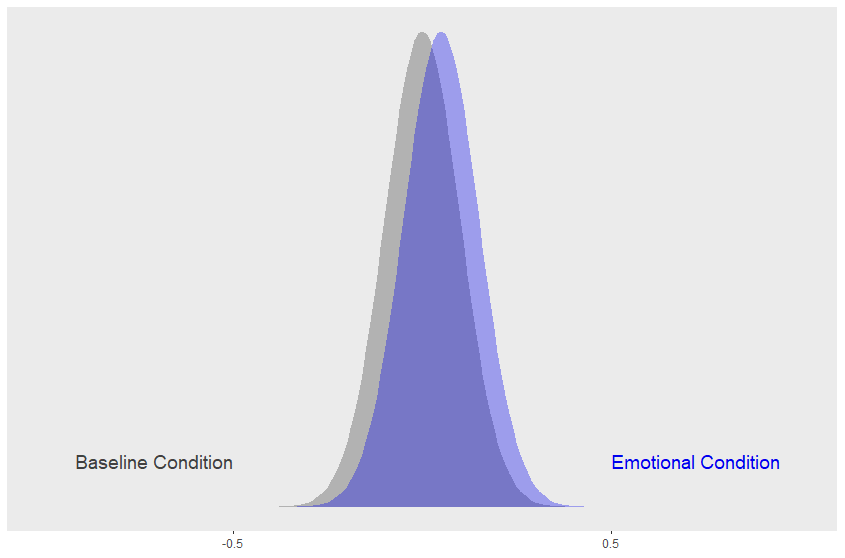
\includegraphics[width = \textwidth]{figures/distributions.png}
        \caption{Overlapping distributions. Here, the underlying distributions for the simulations concerning our power analysis is depicted. The baseline is centered around 0, while the emotional condition is based around 0.05. Both have a standard deviation of 0.1}
        \end{centering}
    \end{figure}
    For a power analysis, we used the reported parameters and their standard deviations from \citeA{nilsson2011jomp} to simulate data.

Estimating power in a Bayesian framework does not have the same standardized formulation as it does in a Frequentist framework (See section: Models and Procedure). We chose to mirror the procedures from the frequentist’s framework by having a threshold of 0.8 as our goal for statistical power. In a Bayesian framework, we take this to correspond to 95\% of the probability mass for the posterior distribution of an effect to not include 0 in 80\% of tests performed. 
It should be noted that the reported parameters in \citeA{nilsson2011jomp} are the medians of the distributions, not the mean. For our intents and purposes, we use the reported median as the mean for our simulated data. 

We based our power analysis on the $\alpha$ parameter, which showed the highest standard deviation out of all the parameters associated with the utility function ($\alpha, \beta, \lambda$). It should be mentioned that we still analyse the other parameters associated with the probability weighting function, but that these showed larger standard deviations. As such, stronger absolute differences from the baseline are required to make sound inferences. 
\citeA{nilsson2011jomp} finds that the standard deviation is highest for the parameter $\alpha$ ($SD = 0.1$). We propose that interesting deviations from the baseline would be deviations of 0.05 (e.g. baseline = 0.88, condition = 0.83). In terms of Cohen’s $d$, this corresponds directly to a medium sized effect (Cohen’s $d = 0.5$). We simulated 100 studies using the ‘R’ package \textit{BRMS}, and found that the posterior distribution of 80\% of these studies did not include 0 with 60 participants. All the code for the simulation is available on the \href{https://github.com/sebsebar/Nature-Study/blob/main/PowerAnalysis/BayesianPower.Rmd}{Github}. 
Importantly, this does mean that for smaller effects, the study will be underpowered. As such, we will not be able to make sound inferences for small effects (Cohen’s $d = 0.2$).

\begin{figure}[H]
    \begin{centering}
    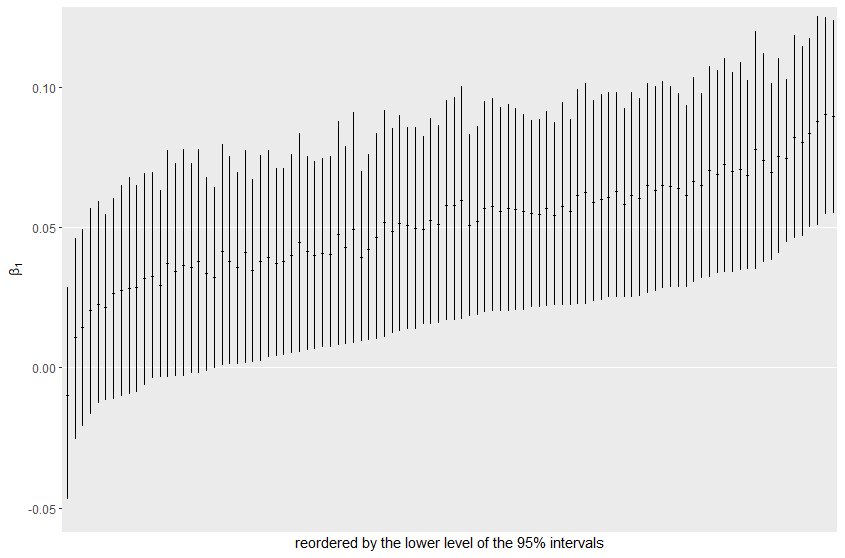
\includegraphics[width = \textwidth]{figures/estimates.png}
    \caption{Plot showing 100 simulations of the estimating the difference between the two groups. Lowest white line indicate 0(baseline), upper indicating 0.1(true effect). Using 60 participants, this corresponds to 80\% of these bars to not include 0 in 95\% of their probability mass}
    \end{centering}
\end{figure}

Although \citeA{nilsson2020jomp} finds reliable parameters using only 30 participants, our power analysis suggests that we need 60 participants per condition to find effects of interest in our study. We assume a rate of 15\% data loss due to poor quality or technical issues. We therefore initially collect 69 participants in each condition. In sum, we collect 345 participants, which are split into 5 different conditions. 
    \subsection{Stopping Rule}

    For the Lab-based study we will stop collecting data once we reach 69 participants or once we run out of rooms, as COBE-Lab will only be able to host our study for a fixed amount of time.

For the online study, we are in full control of the exact sample size, as Qualtrics will allow for continuous access to its cohort. Bearing this in mind we will base our stopping rule for collection of participants on the quality of their data. We cannot ignore the possibility that the online study will have a higher level of erroneous and faulty data. And as the exclusion of participants might affect certain conditions disproportionally, we will allow ourselves to rerun single conditions until the target of 69 participants is met (See the section: exclusion criteria).  This is done to avoid having to rerun the whole study if one condition doesn’t meet the target level of 69 participants.

    \section{Variables}

    \subsection{Manipulated Variables}
    We will manipulate the affective states of our participants in the dimensions of valence and arousal by having them watch selected video material from the meta-analytically reviewed database of AIP stimuli. We use videos that have been shown to reliably induct predefined levels of valence and arousal (See section: Videos). The chosen AIPs will elicit these four affective states: A+V+,A+V-,A-V+,A-V- (See the section: Study Design).

    \subsection{Measured Variables}
    With a trial by trial two-alternative forced-choice paradigm, we will have our participants choose between lotteries in a mixed gamble task. Each choice will be binary and be within one of three block groups: Gains, Losses or Mixed Scenarios.
    Moreover, after having shown the AIP material for each of the four conditions (A+V+,A+V-,A-V+,A-V- (See the section: Study Design)) in each block’s phase 1, we will also have our participants rate their own affective state in regard to arousal (on a scale 1 - calm to 9 -excited) and valence (on a scale 1-unhappy to 9 - happy) using SAM. These scores will be used as a manipulation check.

    \subsection{Indices}
    We will collect reaction times from all our participants to check whether they fulfill our exclusion criteria or not. This entails binning the reaction times into a factor of above and below 100ms (See the section: Exclusion Criteria).
    \section{Analysis Plan}
    \subsection{Statistical models}
    We use bayesian parameter estimation as our statistical model, to estimate the predicted parameter values of Cumulative Prospect Theory for each condition.
As previously stated, Cumulative Prospect Theory is specified as:

$$V(O) = \sum \pi (p_i)v(x_i) $$

Recall that in sum, our probabilistic version of cumulative Prospect Theory is specified by six parameters, each of which being directly interpretable:

\begin{enumerate}
    \item $\alpha$ defines the curvature of the subjective value function in the gain domain;
    \item $\beta$ defines the curvature of the subjective value function in the loss domain;
    \item $\lambda$ defines loss aversion;
    \item $\gamma$ defines the probability weighting function’s shape in the gain domain;
    \item $\delta$ defines the probability weighting function’s shape in the loss domain
    \item $\varphi$ defines to what degree choice behavior is determined by subjective values.
\end{enumerate}
We use and follow the specific coding guidelines for analysis used by \cite{nilsson2011jomp}. Specifically, we will estimate the six parameters using Hierarchical Bayesian Parameter Estimation on the data from each condition separately. This is done to ensure that means are only pooled within each specific condition, and not towards the overall mean of the entire population. Next, we will check the degree to which the data supports our hypotheses by performing simple Bayesian t-tests between the baseline and the condition of interest, and calculate the Bayes Factor associated with the alternative hypothesis. This is done by using the \textit{BayesFactor} package in R. 

    \subsection{Transformations}

    We followed the procedure outlined in \citeA{nilsson2020jomp} regarding transformations and priors for all the parameters of the Hierarchical Bayesian Model. Specifically, we will transform the parameters which are constrained to values between 0 and 1 ($\alpha, \beta, \gamma,\delta$), to a probit scale (a real number line), to make the model converge. For each participant, the individual probitized parameters will be based on a group-level prior, which will be a uniform distribution $N(0,1)$ on the ratescale that goes from 0 to 1.
The two parameters $\lambda$ and $\varphi$ will not need to be transformed. But given that these two parameters are limited to positive values, we will use lognormal distributions for their group-level priors. For these we use an uninformative uniform prior distribution, $U(-2.30, 1.61)$ as also outlined in \cite{nilsson2011jomp}.
For more detailed information see \citeA{nilsson2011jomp}.
    \subsection{Inference criteria}
    Bayesian hypothesis testing will typically yield Bayes factor (BF) values between 0.01 and 100. To this effect we will use the widely adopted Lee and Wagenmakers’ classification scheme, to consider Bayes Factors above 3 and below 0.33 as informative “moderate” effects  \cite{lee2014}. 
In the study we will be using bayesian ANOVAs and/or t-tests. In a two-tailed test we will consider BFs $\geq$ 3 to be indicating support for the alternative hypothesis, BFs $\leq$ 0.33 as indicating support for the null hypothesis and all BFs between 0.33 and 3 will be considered as inconclusive. 
As explained in the intro, we will not correct for the family-wise error.

    \subsection{Data Exclusion}

    We will exclude participants with missing data (e.g. loss of data due to a technical failure) or insufficient data (less than 180 completed trials within a condition). Moreover, we will identify outliers in task performance by examining boxplots of reaction times (RT) across all subjects; subjects whose RT are faster than 100 ms or greater than 3 standard deviations from the median RT will be excluded from the analysis. Moreover, we will exclude any participant who only picks a left or right side gamble, because this indicates that the individual was unable to follow the instructions and perform the two-alternative forced-choice task correctly.

Moreover, SAM scores will be used as stimulus checks and any participants that do not consequently rate their own affective state in correspondence to one of our four conditions (A+V+,A+V-,A-V+,A-V- (See the section: Study Design)) will be excluded. For example,, participants in the condition of high arousal and high valence (A+,V+), we will exclude participants that do not score themselves as being higher than 5 in both dimensions. 5 is the middle point on the SAM scale,which indicates neutrality.

\subsection{Exploratory analysis}

We will also explore whether the inclusion of Gender, Age, Income, Marital Status, Educational Level, Scientific Literacy and Nationality influence the parameter estimates of our hierarchical bayesian models. An example could be that older age would reverse the $\beta$ parameters direction of effect in loss scenarios, indicating that the effect of loss aversion was bigger for the elderly, compared to the young.
Moreover, we will explore how the parameters vary across the two studies (Online and Lab-based), to explore any shift in direction of effects for any of the parameter variables.

As touched on in the introduction, we will also explore the possible effects of negativity bias reported in the meta analysis \cite{joseph2020pbb}. In general, negative emotions have been shown to be more easily elicited in participants than positive emotions, and we find it valuable to investigate if this pattern is replicated in this study in case it would influence what effects we find evidence for.

As touched on in the introduction we have added an error theory to our model specifying the $\varphi$-parameter that quantifies how random the behavior of an individual is. We intend to explore how the $\varphi$-parameter varies across the four conditions.

Lastly, at the end of the experiment, each participant will be inquired whether they know the concept of loss aversion. This will serve as a proxy for a general knowledge of behavioural economics. Like the demographic variables, this measure is not central to any hypothesis, but will be included as a potential signpost if our experiment should face any systematic errors when replicating the baseline model of Cumulative Prospect Theory. 

\subsection{Other}
The reason for our interest in a pre-registered study design, and the Open Science Foundation that will host our materials openly, is first and foremost to achieve a higher level of control over type-I and type-II error rates, as well as secure a better reproducibility of our study. With this in mind we’ll close with the assertion that any minor deviation from the pre-registration that should come about will be documented and outlined before submission to any journal.

    \bibliographystyle{apacite}

    \bibliography{NATURE-PAPER}
\end{document}